\documentclass[11pt,a4paper]{article}
\usepackage[utf8]{inputenc}
\usepackage[T1]{fontenc}
\usepackage{lmodern,amsmath,amssymb,amsthm,mathtools,booktabs,hyperref,enumitem,microtype}
\usepackage[margin=1in]{geometry}
\usepackage{graphicx}
\usepackage{tikz}
\usetikzlibrary{arrows.meta,positioning,calc,fit,backgrounds,patterns}
\usepackage[round,authoryear]{natbib}

\newtheorem{definition}{Definition}[section]
\newtheorem{proposition}[definition]{Proposition}
\newtheorem{hypothesis}[definition]{Hypothesis}
\newtheorem{corollary}[definition]{Corollary}
\theoremstyle{remark}
\newtheorem*{remark}{Remark}

\newcommand{\Frame}{\mathcal F}
\newcommand{\Seldon}{\mathcal S}
\newcommand{\Goal}{\mathcal G}
\newcommand{\Much}{\mathcal M}
\newcommand{\Aset}{\mathcal A}
\newcommand{\Hist}{\mathcal H}
\newcommand{\Qrho}{\mathcal Q_{\rho}}

\title{Seldon Manifolds --- Theory\\\large The Geometry of Reachable Futures}
\author{Matthew Parslow\\Independent Researcher}
\date{\textbf{Draft \textemdash\ draft-2026-08-27}\\[2pt]27 August 2026}

\usepackage{fancyhdr}
\pagestyle{fancy}
\fancyhf{}
\fancyfoot[C]{\thepage}
\fancyfoot[R]{\scriptsize\textsc{draft-2026-08-27}}
\renewcommand{\headrulewidth}{0pt}
\fancypagestyle{plain}{\fancyhf{}\fancyfoot[C]{\thepage}%
  \fancyfoot[R]{\scriptsize\textsc{draft-2026-08-27}}\renewcommand{\headrulewidth}{0pt}}
\begin{document}
\maketitle
\begin{center}
\fbox{\parbox{0.92\textwidth}{\small
\textbf{DRAFT --- draft-2026-08-27} (27 August 2026).
This document is under active revision and is circulated for comment, not as a
finished result. Definitions, numbering and claims may change between drafts;
cite the version string above if referring to it. Sections marked as
falsifiability commitments are the intended points of attack.}}
\end{center}
\vspace{1em}


\begin{abstract}
Graphic Equalisation requires only admissible continuation and deterministic collapse. It does not require a graph or containing frame to represent unrealised futures as an object. This paper studies the additional structure that appears when a frame represents the futures that remain distinguishably reachable under counterfactual admissible interventions and represented future boundary conditions. The resulting object is the \emph{Seldon manifold}: a frame-relative, horizon-relative, resolution-relative representation of reachable future state or history.

The construction is deterministic at substrate level. A Seldon manifold is not a probability distribution over multiple outcomes of one causally complete antecedent. It is a representation of different deterministic continuations obtained under different admissible interventions, future interactions, or unresolved containing conditions represented by the frame. If all causally relevant future conditions and interventions are fixed, the represented continuation collapses to one trajectory.

The manifold need not be smooth or continuous; ``manifold'' denotes structured reachable geometry. Its dimensions are instantiated only where represented, its values are discrete at operative resolution, and its quantisation may change dynamically. Two distinctions are developed at length: what such a projection is a projection \emph{over} --- the \emph{undetermined}, which collapse has yet to fix, as against the \emph{undisclosed}, which is realised but not held by this frame --- and \emph{causal depth}, the additional determining structure supplied by containing frames rather than by earlier times. Goals, where represented, define acceptable subsets; Muchness measures retained distinguishable future possibility; irreversibility removes reachable distinctions; and control deforms the reachable geometry. No primitive is added to graphhood.
\end{abstract}

\section{Scope and relationship to prior work}\label{sec:scope}

Reachable sets, viability kernels, capture basins, invariant sets, dynamic programming, Hamilton--Jacobi reachability, and model-predictive control are established parts of control theory and applied mathematics \citep{bellman1957,aubin1990,aubin1991,mitchell2005,bansal2017,rawlings2017}; this paper claims none of them as new, and its contribution is their placement inside the Graphic Equalisation frame architecture, stated in full in Section~\ref{sec:positioning}.

\section{Dependency on Graphic Equalisation}\label{sec:dependency}

\paragraph{Reading for the claim.}
As in the foundational paper, the components used here are individually established and cited as such; the claim is their arrangement, which is not reachable by evaluating those components separately, since they are stipulated to be known. The composition's own falsifiability commitment is stated in the foundational paper and is inherited here.

Let
\[
G_t=(g_t,r_t,\Gamma_t)
\]
be a realised graph in individuating frame $W_k$, and write
\[
\Frame_{k,t}=(G_t,W_k).
\]
Graphic Equalisation supplies a deterministic realised transition once the causally complete antecedent configuration is fixed. It also distinguishes immediate admissible possibility from realised collapse:
\[
G_t\longrightarrow\Aset(\Frame_t)\xrightarrow{\mathcal C_t}G_{t+1}.
\]

This paper asks what follows when a frame represents recursively reachable continuations over a horizon rather than only the realised next step.

\section{Determinism and counterfactual reachability}\label{sec:determinism}

\begin{proposition}[Deterministic reachability]\label{prop:det-reach}
A Seldon manifold does not require stochastic substrate dynamics. For a fixed causally complete antecedent configuration and a fixed future sequence of admissible interventions and containing interactions, Graphic Equalisation yields one realised continuation. Multiple points or histories in a Seldon manifold correspond to different counterfactual future conditions represented by the frame, not multiple random outcomes of one identical complete cause.
\end{proposition}

Let $\mathbf u=(u_t,\ldots,u_{t+h-1})$ denote an admissible intervention sequence and $\mathbf b=(b_t,\ldots,b_{t+h-1})$ a represented sequence of future boundary conditions or containing interactions. For a deterministic transition law $T$, a future history is generated recursively by
\[
G_{j+1}=T(G_j,u_j,b_j).
\]
The frame need not know which $\mathbf b$ will be realised. Its uncertainty about that sequence may be represented probabilistically if useful, but probability is an epistemic overlay on the reachable family rather than a primitive of the Graph Law.

\begin{corollary}[Singleton under complete fixing]\label{cor:singleton}
If the frame fixes the causally complete antecedent, all future interventions, and all causally operative future containing conditions over horizon $h$, then the Seldon manifold contains one distinguishable continuation at that resolution.
\end{corollary}

This distinction is important because classical reachability and viability theory often permit disturbances, controls, or differential inclusions to generate sets of possible states \citep{aubin1991,mitchell2005}. The Seldon construction can represent the same set-valued geometry without interpreting that set as fundamental stochasticity.

\section{Standing of the construction}\label{sec:standing}

Before the definitions, a boundary on what is being claimed, because the natural reading of what follows is stronger than the position of this paper.

\begin{remark}[Succession does not require an observer]\label{rem:ratchet-first}
Realised change, and the succession its enabling-order carries, exist independently of any frame representing them. Graphic Equalisation withholds even a ratchet-mechanism over the changes --- succession is a relation carried by which change enables which, not an engine the substrate runs --- but that order is substrate-level regardless of any observer. Seldon manifolds, by contrast, are \emph{optional observer or agent machinery} for representing reachable unresolved continuations. Nature does not have to run a Seldon manifold in order to evolve.
\end{remark}

\begin{remark}[The horizon is doubly observer-relative]\label{rem:horizon-observer}
The horizon $h$ is not a substrate quantity. By Graphic Equalisation's Axiom on time, the substrate has succession and no time dimension; a temporal dimension exists only where a frame instantiates one to represent that succession. So $h$ is measured in a dimension the observing frame constructed, and indexes a manifold the same frame constructed. Both the ruler and the thing measured are observer machinery, and neither is a claim about what the world contains.
\end{remark}

\begin{remark}[Higher machinery is frame-relative, not substrate-required]\label{rem:optional-machinery}
The same holds of every construct in this paper and its successors: manifolds, undetermined counts, inferred futures, Narrative, and Narrativium are first-class quantities \emph{only in frames that instantiate the relations defining them}. They are not universal substrate requirements, and their absence from a frame is not a deficiency of that frame's dynamics.
\end{remark}

These remarks are load-bearing for the falsifiability commitments in Section~\ref{sec:falsifiability}: a claim about what an agent's representation supports is not a claim about what the world must contain.

\section{Dimensions, values, and resolution}\label{sec:dimensions}

\begin{definition}[Represented dimension]\label{def:dimension}
A dimension $D$ of a Seldon representation exists in frame $\Frame$ only where the frame instantiates the relation needed to distinguish values along $D$. If that relation is absent, $D$ is undefined in that frame; it is not present with value zero.
\end{definition}

Thus
\[
D:\operatorname{NULL}\longrightarrow D\in\Frame
\]
is a dimensional instantiation, whereas
\[
D=0
\]
is a value statement made only after $D$ exists. This preserves the dimension/value distinction established by Graphic Equalisation.

\begin{definition}[Resolution]\label{def:resolution}
Resolution $\rho$ specifies which distinctions on instantiated dimensions the frame currently treats as distinguishable in represented future structure.
\end{definition}

Resolution is discrete but may vary dynamically:
\[
\rho=\rho(x,h,t,D).
\]
No globally fixed lattice, common scale, or continuous coordinate system is assumed. A grounding may map integer state indices into arbitrary physical scales.

Let $\sim_{\rho}$ denote ``indistinguishable at resolution $\rho$''. The quotient
\[
\Qrho(X)=X/{\sim_{\rho}}
\]
collects states or histories into the distinctions the frame can currently resolve.

\begin{remark}[These are the aperture, decomposed]\label{rem:aperture}
What the foundational papers call a frame's \emph{aperture} --- the bound on what it can distinguish
at all --- appears here under several names rather than one. The horizon $h$ bounds how far forward
it reaches, the resolution $\rho$ how finely it separates what it reaches, and the represented
dimension set which properties it can separate along; a blind spot (Definition~\ref{def:blind-spot})
is a further deficit again, and not a coarser reading of the same one
(Remark~\ref{rem:two-deficits}).

The decomposition is deliberate and should not be collapsed back. An aperture is not one dial: two
frames may match on resolution and differ on horizon, or share both and differ on which dimensions
they instantiate at all, and those are different limitations with different consequences. Different
agents accordingly hold different manifolds of the same situation --- not better and worse
approximations to one manifold, since there is no frame-free manifold for them to approximate.

This extends to everything defined over a manifold and not only to its extent. A field is defined
where the frame instantiates the dimension it is a field of, and is \textsc{null} elsewhere rather
than large, so two frames may agree on which futures are reachable and still disagree on what those
futures cost, or on whether cost is a thing they represent at all.
\end{remark}

\section{The Seldon manifold}\label{sec:seldon}

\begin{definition}[Seldon manifold]\label{def:seldon}
For frame $\Frame_t$, horizon $h$, and resolution $\rho$, the Seldon manifold
\[
\boxed{\Seldon_{h,\rho}(\Frame_t)}
\]
is the structured representation, at resolution $\rho$, of future states or histories reachable from $\Frame_t$ over horizon $h$ under the admissible counterfactual intervention sequences and represented future containing conditions carried by that frame.
\end{definition}

Equivalently, if $\mathcal U_{t:h}$ is the represented family of admissible intervention sequences and $\mathcal B_{t:h}$ the represented family of future boundary-condition sequences, then schematically
\[
\boxed{
\Seldon_{h,\rho}(\Frame_t)
=
\Qrho\!\left(
\left\{
\Hist_{t:t+h}(\mathbf u,\mathbf b):
\mathbf u\in\mathcal U_{t:h},\;
\mathbf b\in\mathcal B_{t:h}
\right\}
\right).
}
\]

The term \emph{manifold} is operational rather than differential-geometric. Depending on the grounding, $\Seldon$ may be represented as a reachable set, graph, viability kernel, capture basin, branching history structure, automaton, cell complex, or another object preserving the relevant reachability relations. Viability kernels and reachable sets are therefore direct mathematical predecessors \citep{aubin1990,aubin1991,szolnoki2000,mitchell2005}.

\begin{proposition}[Immediate possibility is not future geometry]\label{prop:local-vs-manifold}
$\Gamma_t$ constrains local admissibility, whereas $\Seldon_{h,\rho}(\Frame_t)$ represents recursively reachable structure over a non-zero horizon. The two coincide only in a grounding where the chosen horizon and representation reduce reachability to one local transition.
\end{proposition}

\section{Projection and recursion}\label{sec:projection}

The Seldon manifold may be viewed as a projection of recursively composed admissible transitions, but the future transition structure must be generated from each counterfactual successor rather than read as though the actual future were already known. Thus a schematic recursion is
\[
\Seldon_{h+1,\rho}(\Frame_t)
=
\Qrho\!\left(
\bigcup_{\delta\in\Aset(\Frame_t)}
\operatorname{Extend}
\left(
\delta,
\Seldon_{h,\rho}(\Frame_{t+1}^{(\delta)})
\right)
\right),
\]
with boundary contingencies included in $\delta$ or in the successor frame as required by the grounding.

This is extensional. It does not require an implementation to enumerate every individual trajectory. Dynamic programming already exploits recursive state structure rather than recomputing complete histories independently \citep{bellman1957}; set-based reachability methods similarly represent families of trajectories through shared geometric structure \citep{mitchell2005,bansal2017}.

\section{Dynamic quantisation and temporal foveation}\label{sec:foveation}

\begin{hypothesis}[Adaptive resolution]\label{hyp:adaptive-resolution}
For bounded representation, an effective future model assigns finer distinction where additional resolution materially changes reachable, acceptable, or controllable outcomes, and coarser distinction where refinement would not alter any operative decision.
\end{hypothesis}

Thus $\rho(x,h,D)$ may increase where unresolved distinctions become decision-relevant. Near and distant horizons may use different quantisation, as may relevant and irrelevant spatial, causal, or conceptual regions. New dimensions may also be instantiated when a previously absent distinction becomes operative; this is not a change from value zero but a change in representational dimension.

Adaptive mesh refinement provides an established computational analogue: resolution is recursively concentrated where local error estimates justify the additional cost \citep{berger1984}. The Seldon hypothesis differs in criterion---decision relevance rather than numerical truncation error---but shares the principle that uniform resolution is not mandatory.

The efficiency reading above is the weaker of two, and the stronger one is what the rest of this
paper rests on. A frame at resolution $\rho$ does not occupy a point that it represents coarsely; it
occupies a cell, and at its own grain there is no finer fact about where it is. Its destination is a
region in the same sense --- movement is toward \emph{there}, not to a coordinate --- which is why
the acceptable manifold was a region from the outset rather than a target with a tolerance band.

The distinction from a probabilistic reading matters and is easily lost. A distribution over states
represents uncertainty about a point that exists; a cell represents the absence of a finer fact at
that grain. The first has a hidden variable and the second does not, and only the first can be
resolved by observation alone.

This is where a static discretisation would fail the construction, and where the analogy to adaptive
mesh refinement stops. A mesh refines toward a solution that exists independently of it, with error
measured against that solution; a fixed grain is likewise always a grain \emph{relative to}
something finer, so the question ``coarse compared to what'' has an answer, and that answer restores
the observer-free object this construction denies. Dynamic quantisation removes the referent rather
than approximating it: the grain is set by what a frame cannot absorb --- residual driving
subdivision, per dimension, as Graphic Equalisation's growth ladder does --- so the cells are
generated by the frame's own encounter with what exceeds it, not sampled from an assumed underlying
continuum. There is then nothing for a region to be an approximation to, which is what allows two
frames to hold genuinely different manifolds of one situation rather than differently-accurate
approximations to a manifold neither of them has.

\section{Unresolved structure, and the present as a limit}\label{sec:unresolved}

Graphic Equalisation distinguishes four states of a dimension in a frame: NULL (not instantiated), undetermined (instantiated, no value realised), undisclosed (realised, not held by this frame), and resolved. That distinction is what the horizon-dependence of a Seldon manifold is actually about, and \emph{which} of the two middle states is at issue determines which object one is talking about.

\begin{definition}[Undetermined count]\label{def:unknown-count}
For frame $\Frame$ and projected horizon $h$, let
\[
U_{\Frame}(h)
\]
be the number, or more generally the structure, of instantiated \emph{undetermined} dimensions in the frame's projection at that horizon --- dimensions for which no value has been realised. NULL dimensions are excluded, being no variables at all; \emph{undisclosed} dimensions are also excluded, being already determined.
\end{definition}

\begin{remark}[A manifold and a blind spot are different deficits]\label{rem:two-deficits}
A Seldon manifold is a projection over the \emph{undetermined}: it represents continuations that have not been realised, and its width is the structure of what collapse has yet to fix. A blind spot (Definition~\ref{def:blind-spot}) is a limitation over the \emph{undisclosed}: the value exists and this frame does not hold it.

The two are frequently conflated under ``uncertainty'' and behave differently under every operation that matters. Undisclosed structure can be obtained --- by observation, by another frame's report, or by inference from surrounding relations. Undetermined structure cannot be obtained by any of those, because there is nothing yet to obtain; it is settled only by collapse. A frame that improves its access reduces the second and leaves the first untouched.
\end{remark}

\begin{proposition}[The present is $U_{\Frame}=0$]\label{prop:present-limit}
The present is the collapse boundary at which every instantiated undetermined dimension relevant to that collapse has been determined,
\[
\boxed{U_{\Frame}=0,}
\]
and as the projected horizon approaches the present,
\[
U_{\Frame}(h)\longrightarrow 0 .
\]
\end{proposition}

Future distance in a Seldon manifold is therefore not merely geometric resolution. The operative quantity is \emph{undetermined} structure --- not what the frame has failed to observe, but what has not yet been settled.

\begin{definition}[Observer-relative determinability]\label{def:determinability}
Let $D_{\Frame}(h)$ be the fraction, or measure, of determining structure resolved in-frame at horizon $h$, with
\[
\lim_{h\to0^{+}}D_{\Frame}(h)=1,
\qquad
D_{\Frame}(0)=1 .
\]
\end{definition}

\begin{remark}[What is changing, and what is not]\label{rem:not-more-deterministic}
The Graph Law is deterministic throughout, at every horizon. What varies with $h$ is how much determining structure is \emph{resolved in-frame}. It is therefore incorrect to say that the universe becomes more deterministic as the present is approached; determinism is not a quantity that varies. The observer's determinability does.
\end{remark}

Consistently with Graphic Equalisation's distinction between \emph{determinable} and \emph{determined}, a continuation may be fully determinable from present structure without having been realised. The manifold represents determinable continuations; collapse produces determined ones.

\begin{definition}[Blind spot]\label{def:blind-spot}
A frame may fail to observe a projected region directly while still constraining its continuation through relations around it. Three states must therefore be distinguished:
\[
\boxed{\text{directly resolved}\;\neq\;\text{unresolved}\;\neq\;\text{occluded but inferable}.}
\]
\end{definition}
A blind spot is a limitation of access, not a hole in reality, and an occluded-but-inferable region is not epistemically equivalent to an unapproached one. Collapsing the two discards the surrounding constraint.

All three states in Definition~\ref{def:blind-spot} concern the \emph{undisclosed}: in each case a value has been realised and the question is only how much of it this frame can reach. None of them is a statement about the undetermined, and a projection that mixes the two will report a manifold width that no amount of observation could ever reduce, or an occlusion that no observation could ever resolve.

\section{Reachability rather than point prediction}\label{sec:prediction}

Point prediction seeks
\[
\widehat{\Frame}_{t+h}\approx\Frame_{t+h}.
\]
The Seldon formulation instead asks which futures remain reachable under the represented counterfactual family:
\[
\Frame_{t+h}\in\Seldon_{h,\rho}(\Frame_t).
\]

This emphasis is close to viability and Hamilton--Jacobi reachability, where the central objects are sets of states that can remain safe, reach targets, or avoid undesirable regions under admissible inputs \citep{aubin1991,mitchell2005,bansal2017}. A point forecast can still be useful, but it is a statistic or selected continuation over the reachable structure rather than the primary object.

\section{Acceptable futures}\label{sec:acceptable}

Goals are optional represented capabilities.

\begin{definition}[Acceptable manifold]\label{def:acceptable}
Where a frame represents goals, viability conditions, risk bounds, or constraints,
\[
\boxed{\Goal_{h,\rho}(\Frame_t)\subseteq\Seldon_{h,\rho}(\Frame_t)}
\]
is the subset of reachable futures satisfying them.
\end{definition}

This overlaps directly with viability kernels and feasible regions in constrained control and model-predictive control \citep{aubin1991,rawlings2017,cunis2021}. The Seldon terminology is broader because the acceptable subset may be defined over any represented future distinctions, not only a conventional continuous state space.

Figure~\ref{fig:tube} draws the construction.

\begin{proposition}[Minimum intervention in a safe interior]\label{prop:min-intervention}
Suppose the represented no-intervention alternative exists and its continuation remains within the acceptable manifold over the decision horizon. If every non-trivial intervention has non-negative cost and no independent objective rewards intervention itself, then a positive-cost intervention cannot dominate the no-intervention alternative solely by preserving acceptability.
\end{proposition}

\begin{remark}
``No intervention'' here is an instantiated alternative with a defined consequence, not NULL (Definition~\ref{def:dimension}); the proposition does not identify absence with a zero-valued action.
\end{remark}

\begin{figure}[t]
\centering
\resizebox{\textwidth}{!}{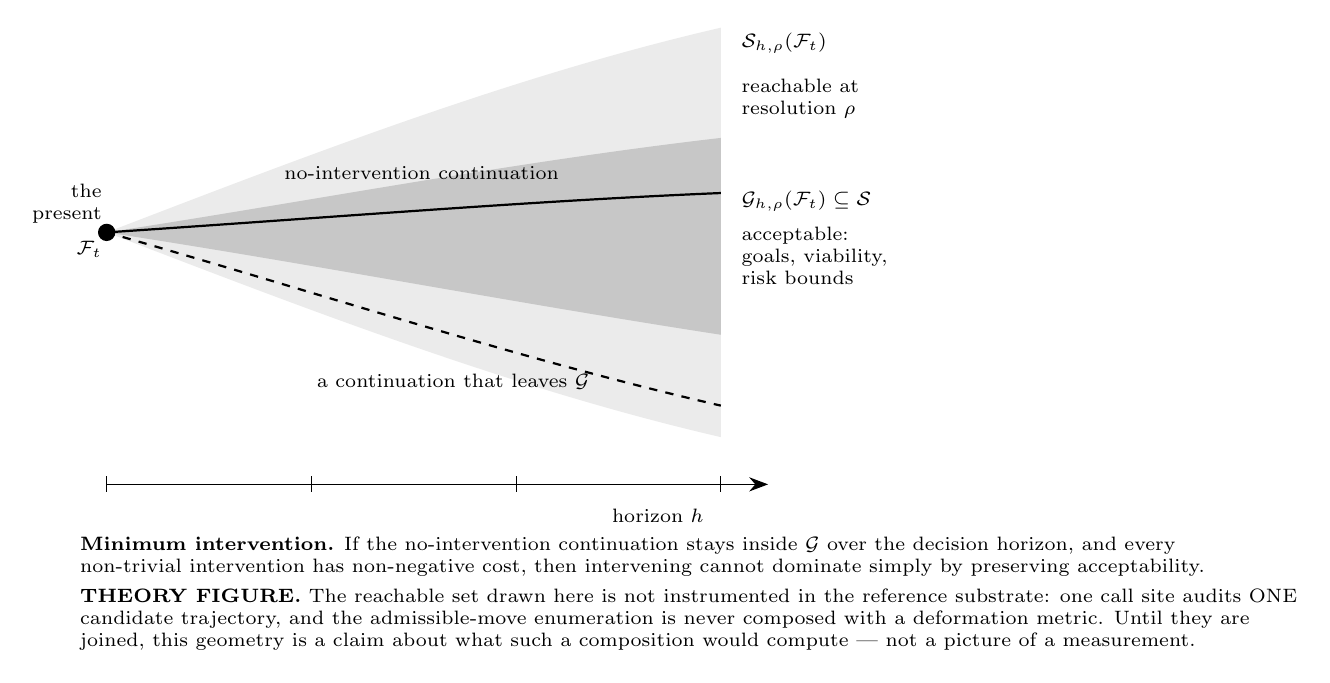
\begin{tikzpicture}[
  >={Stealth[length=2.4mm]},
  lbl/.style={font=\scriptsize, inner sep=1.6pt},
  hist/.style={thick},
  x=1mm, y=1mm,
]
% --- the reachable set, widening with horizon --------------------------
\fill[black!8]
  (0,0)
  .. controls (26,10) and (52,20) .. (78,26)
  -- (78,-26)
  .. controls (52,-20) and (26,-10) .. (0,0) -- cycle;
\node[lbl, anchor=west] at (80,24) {$\mathcal{S}_{h,\rho}(\mathcal{F}_t)$};
\node[lbl, anchor=west, align=left] at (80,17)
  {reachable at\\resolution $\rho$};

% --- the acceptable subset --------------------------------------------
\fill[black!22]
  (0,0)
  .. controls (26,4) and (52,9) .. (78,12)
  -- (78,-13)
  .. controls (52,-9) and (26,-4) .. (0,0) -- cycle;
\node[lbl, anchor=west] at (80,4) {$\mathcal{G}_{h,\rho}(\mathcal{F}_t)\subseteq\mathcal{S}$};
\node[lbl, anchor=west, align=left] at (80,-3)
  {acceptable:\\goals, viability,\\risk bounds};

% --- the present frame -------------------------------------------------
\fill (0,0) circle (1.1);
\node[lbl, below left=0.5mm and 0mm of {(0,0)}] {$\mathcal{F}_t$};
\node[lbl, above left=0.5mm and 0mm of {(0,0)}, align=right] {the\\present};

% --- two continuations -------------------------------------------------
\draw[hist] (0,0) .. controls (30,2) and (54,4) .. (78,5);
\node[lbl, anchor=west, black] at (78.5,5.6) {};
\node[lbl] at (40,7.5) {no-intervention continuation};

\draw[hist, dashed] (0,0) .. controls (28,-8) and (52,-16) .. (78,-22);
\node[lbl] at (44,-19) {a continuation that leaves $\mathcal{G}$};

% --- the horizon axis --------------------------------------------------
\draw[->] (0,-32) -- (84,-32);
\node[lbl] at (70,-36) {horizon $h$};
\foreach \x in {0,26,52,78}{\draw (\x,-31) -- (\x,-33);}

% --- the proposition, where it bites ----------------------------------
\node[lbl, anchor=north west, align=left] at (-4,-38)
  {\textbf{Minimum intervention.} If the no-intervention continuation stays
   inside $\mathcal{G}$ over the decision horizon, and every\\
   non-trivial intervention has non-negative cost, then intervening cannot
   dominate simply by preserving acceptability.\\[1mm]
   \textbf{THEORY FIGURE.} The reachable set drawn here is not instrumented in
   the reference substrate: one call site audits ONE\\
   candidate trajectory, and the admissible-move enumeration is never composed
   with a deformation metric. Until they are\\
   joined, this geometry is a claim about what such a composition would
   compute --- not a picture of a measurement.};
\end{tikzpicture}
}
\caption{The Seldon manifold, its acceptable subset, and the minimum-intervention
proposition. The reachable set is a representation a frame may construct
(Remark~\ref{rem:ratchet-first}), not a structure the world contains.}
\label{fig:tube}
\end{figure}

\section{Goal direction}\label{sec:goal-direction}

Where local direction is meaningful, let $\mathbf g_t$ be a represented preferred direction through the acceptable region. A grounding may write
\[
\mathbf v_{\Seldon}\cdot\mathbf g_t>0
\]
for progress. No differentiable structure is required by the substrate; a graph grounding may instead use an ordering or directed edge relation.

\section{Cost contours and basins}\label{sec:contours}

The manifold as defined says which continuations are reachable. It does not say that they are
equally easy, and they are not. A manifold therefore admits a scalar field over it --- a cost
assigned to each represented continuation --- and the geometry of that field is as informative as
the extent of the manifold itself. What the scalar \emph{is} is supplied by the companions --- Narrative Momentum, where surviving
history-bearing structure prices continuations rather than removing them, and Narrativium, where the
capacity to pay is itself a frame-relative quantity --- the present paper needs only that some such
field exists over $\Seldon_{h,\rho}(\Frame_t)$ and is frame-relative in the same way the manifold is.

\begin{definition}[Cost field and contours]\label{def:contours}
Where the frame instantiates the relevant dimension, let $C_{\Frame}$ assign to each continuation in
$\Seldon_{h,\rho}(\Frame_t)$ the cost, in that frame's terms, of reaching it; where it does not, the
field is \textsc{null} there rather than large (Definition~\ref{def:dimension}). Its sublevel sets
$\{C_{\Frame}\le k\}$ are the within-budget regions and their boundaries the \emph{contours}. A
\emph{basin} is a region whose cheapest successors lie within it, so that leaving costs more than
remaining.
\end{definition}

Two properties make this more than a way of drawing the manifold. The first is that the field has a
default direction of travel, and the reason is not that doing nothing is free. It is the companion
law's: continuations reusing surviving structure are the cheapest ones, and that structure carries
the frame along rather than holding it at a point, so a frame that does nothing is carried down its
cheapest continuation rather than staying put. The descent is where the narrative goes. This is a
pattern the foundational paper holds at the strength the evidence supports rather than a universal
of the substrate. Contours therefore make a projection visible that the bare reachable set does not --- not
which futures are possible, which is the manifold's extent, but which are \emph{cheap}, which is
its shape.

The second is that basins are where the substrate's persistence phenomena live. A frame inside a
basin will return to it under every cheap continuation, and will leave only by paying the ridge; the
structural lock-in of the companion account is a basin read from above, and the horizon is the
contour beyond which the required payment exceeds what the frame has. Whether a basin holds a given
frame is therefore not a property of the basin alone but of the basin against that frame's capacity,
which is why the same landscape confines one frame and not another.

Two consequences worth stating. Deformation, in the sense of the control section below, re-shapes
this field rather than moving within it, which is a larger change than moving a frame at fixed cost.
And a frame with enough capacity is not confined by any basin the landscape contains --- basins say
where the cheap path runs, never where a frame must go.

A cost field alone is not the whole of it, and taking any fixed set of fields for the whole is the
error the construction most invites. A manifold carries as many fields as the frame instantiates
over it, and which ones those are is a fact about the frame's requirements rather than about the
substrate --- the same optional-machinery discipline that governs represented dimensions generally
(Remark~\ref{rem:optional-machinery}). What follows names three that the companion papers supply,
because they are the ones the rest of this account uses; the set is illustrative and not closed.

Cost is a flow --- what reaching a continuation takes --- while what may matter equally is the state
left behind it: write $K_{\Frame}$ for the capacity a frame expects to have \emph{after} arriving,
where that capacity is instantiated.

The two fields collapse into one wherever capacity is purely depletive, so that what remains is
what was held less what was spent. The companion account establishes no such law and exhibits
transitions that net-gain, so the fields are not in general reducible to one another --- though it
also names groundings that do supply a conserved accounting, and there the two coincide. The
construction below is stated for the groundings where they do not. What their divergence buys is the
representation of two cases a single field cannot carry: an expensive continuation that raises
capacity, and a cheap one that lowers it.

\begin{definition}[Trap]\label{def:trap}
For frame $\Frame$, a \emph{trap} is a basin of $C_{\Frame}$ on which $K_{\Frame}$ is decreasing ---
the cost descent and the capacity descent run together. A basin is a place the cheap path returns
to; a trap is a basin whose occupancy erodes the means of leaving it, which is a property of the two
fields jointly and not of the cost field's asymmetry alone.
\end{definition}

Two consequences follow, and they are the practical content of the section. Descent on cost alone is
the wrong policy on a two-field landscape: it is greedy, and a frame that can look further will pay a
ridge to reach a position of higher capacity, which is a move the cost field alone represents as
simply worse. And the reversibility preference stated below acquires its reason here --- a reversible
action is one that preserves capacity, so preferring reversibility is preferring the second field
where the first is indifferent, which is why the preference is not merely caution.

So far the landscape has been something to read. The point of the construction is that it is also
something to change: a frame does not only descend a field, it re-shapes the field others descend,
and the control section below treats that as the primary operation rather than an afterthought.
Representing it needs one more thing, because contours show where the narrative goes and say nothing
about which parts of the terrain will move.

\begin{definition}[Deformability]\label{def:deformability}
For frame $\Frame$, the \emph{deformability} of a region of its manifold is the cost, in that
frame's terms, of altering the fields over that region --- of changing what continuations there
cost, or what capacity they leave. Write it $\partial_{\Frame}$: a field in its own right over the
same manifold, under the same instantiation condition,
and like the others it is frame-relative: it measures what this frame can move, not what is movable.
\end{definition}

This is the structure one level up. Changing a landscape is priced, and changing what it costs to
change a landscape is priced again; each level is defined whether or not anything can reach it. What
finite capacity bounds is not which levels exist but which a frame can act at, so the regress is
operationally truncated rather than definitionally terminated --- and a frame instantiating no
capacity dimension at all has no economy here to truncate it.

What the third field makes visible is \emph{leverage}. The interesting locations are not where the
terrain is most dramatic but where deformability is low and the effect on the descent is large ---
a ridge that can be lowered cheaply and re-routes everything below it, or a basin whose lip can be
breached at a price some frame can pay. That ratio --- small outlay to large change in where the
narrative runs --- is the companion account's loading lever seen as a location: what is injected is
expensive for the container to re-cohere, and cheap only relative to that response. Where a grounding supplies a cost ordering over
interventions, it is the companion's minimum revision cost that any minimality claim ranges over;
deformability prices something else --- altering the field rather than acting within it --- and the
two should not be run together.

Two things this does not license. Regions of high deformability cost are not immovable --- they are
expensive relative to a given frame's capacity, and another frame, or the same one later, may reach
them; the field records a price, not a prohibition --- prohibition is admissibility's business
(Definition~\ref{def:irreversible}), not cost's. And competing deformation, in the section
below, is competition over this field rather than over position: two frames re-shaping the same
region are not moving a contested object between them but disagreeing about what the terrain should
cost, which is why the contest is decided at the ridges rather than at the point either occupies.

Honest boundary: this is a claim about the \emph{shape} of the fields and not their values. Where the basins lie relative to a frame's capacity, where the two
fields diverge, which ridges separate them, and which way the descent runs are the content; the metric that would put numbers on the contours is supplied by a grounding,
if it is available at all, and nothing here asserts that the field is computable for a given system.
Nor does the field add anything to the manifold's extent: a continuation priced beyond any available
capacity remains reachable in principle and is excluded by cost, not by admissibility, which is the
distinction the companion law turns on.

\section{Muchness}\label{sec:muchness}

\begin{definition}[Muchness]\label{def:muchness}
Muchness
\[
\boxed{\Much(\Frame_t;h,\rho)\in\mathbb Z}
\]
is a frame-relative discrete measure of materially distinguishable future possibility retained within $\Seldon_{h,\rho}(\Frame_t)$.
\end{definition}

A grounding supplies a discrete measure
\[
\mu_{\Much}:\Qrho(\Seldon)\rightarrow\mathbb Z
\]
that preserves the distinctions relevant to the claimed domain. It may count distinguishable states, equivalence classes, connected reachable regions, retained capability classes, or use another integer index. Muchness therefore measures \emph{how much distinguishable future remains}, not how strongly the frame can alter that future.

\begin{proposition}[Resolution and dimension dependence]\label{prop:muchness-resolution}
Muchness is not meaningful without the frame, represented dimensions, horizon, and resolution that determine which future distinctions exist and which count as distinct.
\end{proposition}

The term \emph{Muchness} and its role are specific to this framework. Classical reachable-set and viability theory provide the geometry from which such a measure can be constructed but do not identify this quantity under that name.

\section{Irreversibility}\label{sec:irreversibility}

\begin{definition}[Irreversible contraction]\label{def:irreversible}
An intervention is irreversible relative to frame, horizon, dimensions, and resolution when it makes previously distinguishable valuable future regions unreachable and no admissible continuation within the stated horizon restores them.
\end{definition}

Where the Muchness dimension is instantiated before and after the intervention, a simple discrete contraction measure is
\[
I_{\Frame}(u)=\max\!\left(0,\Much_t-\Much_{t+1}^{(u)}\right).
\]
Here $0$ is a legitimate value on an existing irreversibility dimension, not absence of the dimension (Definition~\ref{def:dimension}).

The option value of preserving reversible choices under uncertain future information has a long history in economics \citep{arrow1974,henry1974,dixit1994}. The present definition is more primitive: it identifies irreversibility structurally with loss of reachable distinctions. No substrate-level probability distribution is required. If a frame overlays probabilities on unresolved future conditions, an expected irreversibility statistic is an epistemic derived quantity, not part of the deterministic Graph Law.

\begin{proposition}[Reversibility preference]\label{prop:reversibility}
If two interventions achieve the same represented objective to equivalent tolerance and otherwise differ only in that one preserves a strict superset of potentially valuable future distinctions, any represented valuation assigning non-negative value to retained optionality weakly prefers the more reversible intervention.
\end{proposition}

\section{Control as manifold deformation}\label{sec:control}

\begin{definition}[Control]\label{def:control}
Where intervention is represented, control is deformation of reachable future geometry:
\[
u:\Seldon\mapsto\Seldon'.
\]
\end{definition}

A controller need not predict one exact future trajectory. It may succeed by deforming reachable geometry so that realised collapse remains inside an acceptable region while preserving useful future distinctions. This set-oriented view is close to viability regulation, reachability-based safety control, and constrained model-predictive control \citep{aubin1991,mitchell2005,rawlings2017,cunis2021}.

\section{Competing deformation}\label{sec:competing}

Several processes may shape one shared Seldon manifold. A local additive approximation
\[
\Delta\Seldon\approx\sum_i\Delta\Seldon_i
\]
may be useful where interactions are approximately separable. More generally,
\[
\Delta\Seldon=\Phi(u_1,\ldots,u_n;G,\Gamma,W).
\]
Dynamic-game reachability provides established mathematics for reachable sets under interacting or adversarial controls \citep{mitchell2005}. The Seldon statement is more general and does not require zero-sum or game-theoretic valuation.

This shared-arena case differs from one graph individuated by several frames: each individuating frame carries its own represented dimensions, resolution, and reachable geometry unless a containing relation explicitly couples them.

\section{Reachability compression}\label{sec:compression}

Let $\{\gamma_i\}$ be an explicit family of trajectories.

\begin{hypothesis}[Reachability compression]\label{hyp:compression}
For task classes in which many trajectories are equivalent with respect to the operative distinctions at resolution $\rho$, a representation of their shared reachable geometry can have lower decision-relevant description complexity than explicit trajectory enumeration:
\[
L(\Seldon)\ll L(\{\gamma_i\}).
\]
\end{hypothesis}

This hypothesis is compatible with the general minimum-description-length principle that useful models exploit shared regularity rather than restating each observation independently \citep{rissanen1978}. It is also reflected constructively in set-based reachability methods, which compute or approximate reachable regions without storing every individual trajectory \citep{mitchell2005,maidens2013}. The stronger claim that Seldon representations systematically achieve lower \emph{decision-relevant} description cost is specific to this paper and remains falsifiable.

\section{Relationship to Narrativium and Narrative}\label{sec:downstream}

The present paper distinguishes retained distinguishable future possibility ($\Much$) from the capacity to deform it ($N$); the contrast is set out in full in the companion Narrativium paper, which develops $N$. Narrative is also unnecessary for defining $\Seldon$, but where a containing frame carries operative history-bearing state, that state may orient the manifold; this is the subject of Narrative Momentum.

\section{Causal depth is not temporal distance}\label{sec:depth}

The ordinary picture of time,
\[
\text{history}\rightarrow\text{now}\rightarrow\text{future},
\]
is misleading as a picture of what determines a continuation, and the correction is structural rather than presentational.

Determination has two components. One is \emph{succession}: the order realised changes carry through their enabling-relations, which is what makes a time dimension meaningful at all. The other is \emph{structural depth}: relations instantiated in containing frames, which are present now and are not earlier in time.

Figure~\ref{fig:tilt} contrasts the two pictures directly.

\begin{remark}[The tilt]\label{rem:tilt}
Replacing time by structure entirely would be a $90^{\circ}$ rotation of the causal picture and is not what is claimed. The correct adjustment is closer to a $45^{\circ}$ change of causal vector: succession still runs, and additional determining structure is reached by depth rather than by reaching further back.
\end{remark}

\begin{remark}[No dependent clocks: a subframe need not be slaved to its container]\label{rem:no-dependent-clocks}
Because depth and succession are orthogonal, structural containment carries no temporal subordination. A frame's time is its own change-count (Graphic Equalisation, Axiom on time), and with no global clock there is nothing for a contained frame's clock to be slaved to; each frame counts its own changes. The intuition that a contained process runs \emph{within} its container's time is the assumption of a dependent clock, and it is a property of embodiments that happen to share one, not a substrate fact. Consequently a subframe can run \emph{faster} than its superframe --- accumulate more proper time over the same stretch --- when more of the fixed change-budget falls in it. This does not exceed $c$: the change-rate $c$ is the same in every frame (Graphic Equalisation, $c$ as the change-to-time rate), and what is free is the \emph{ratio} of change-counts between frames, the distribution of the budget across regions, not the per-change rate. A gravitational subframe's ratio is bounded by its physics and a computational subframe's by its throughput; the substrate imposes no dependent-clock law, and the achievable ratio is an engineering fact of the embodiment.

The complement holds equally, and completes the picture: dependence is not \emph{forbidden} either. A subframe \emph{may} be driven --- ticked by a containing frame, and by one several levels above it --- so its clock is then slaved to that superframe's; this is the coupled, locally synchronous case, and it is a coupling paid for, not a substrate necessity. Clock-coupling between a subframe and a container is therefore a free parameter running from fully independent (asynchronous) to fully ticked (synchronous), and nothing compulsory fixes where a given subframe sits. Reality samples the whole range, which is Graphic Equalisation's globally-asynchronous, locally-synchronous structure read on the clock: bound and driven subframes are ticked; uncoupled ones run their own change.
\end{remark}

\begin{proposition}[Depth comes from superframes, not from historical frames]\label{prop:superframes}
Where a continuation is determinable beyond what $\Frame_0$ resolves, the additional determining structure is supplied by containing frames
\[
\Frame_0\subset\Frame_1\subset\Frame_2\subset\cdots,
\]
potentially without a privileged terminal frame. It is \emph{not} supplied by retained temporal snapshots: by Graphic Equalisation's history principle, past states influence the present only where they survive as present structure.
\end{proposition}

\begin{figure}[t]
\centering
\resizebox{\textwidth}{!}{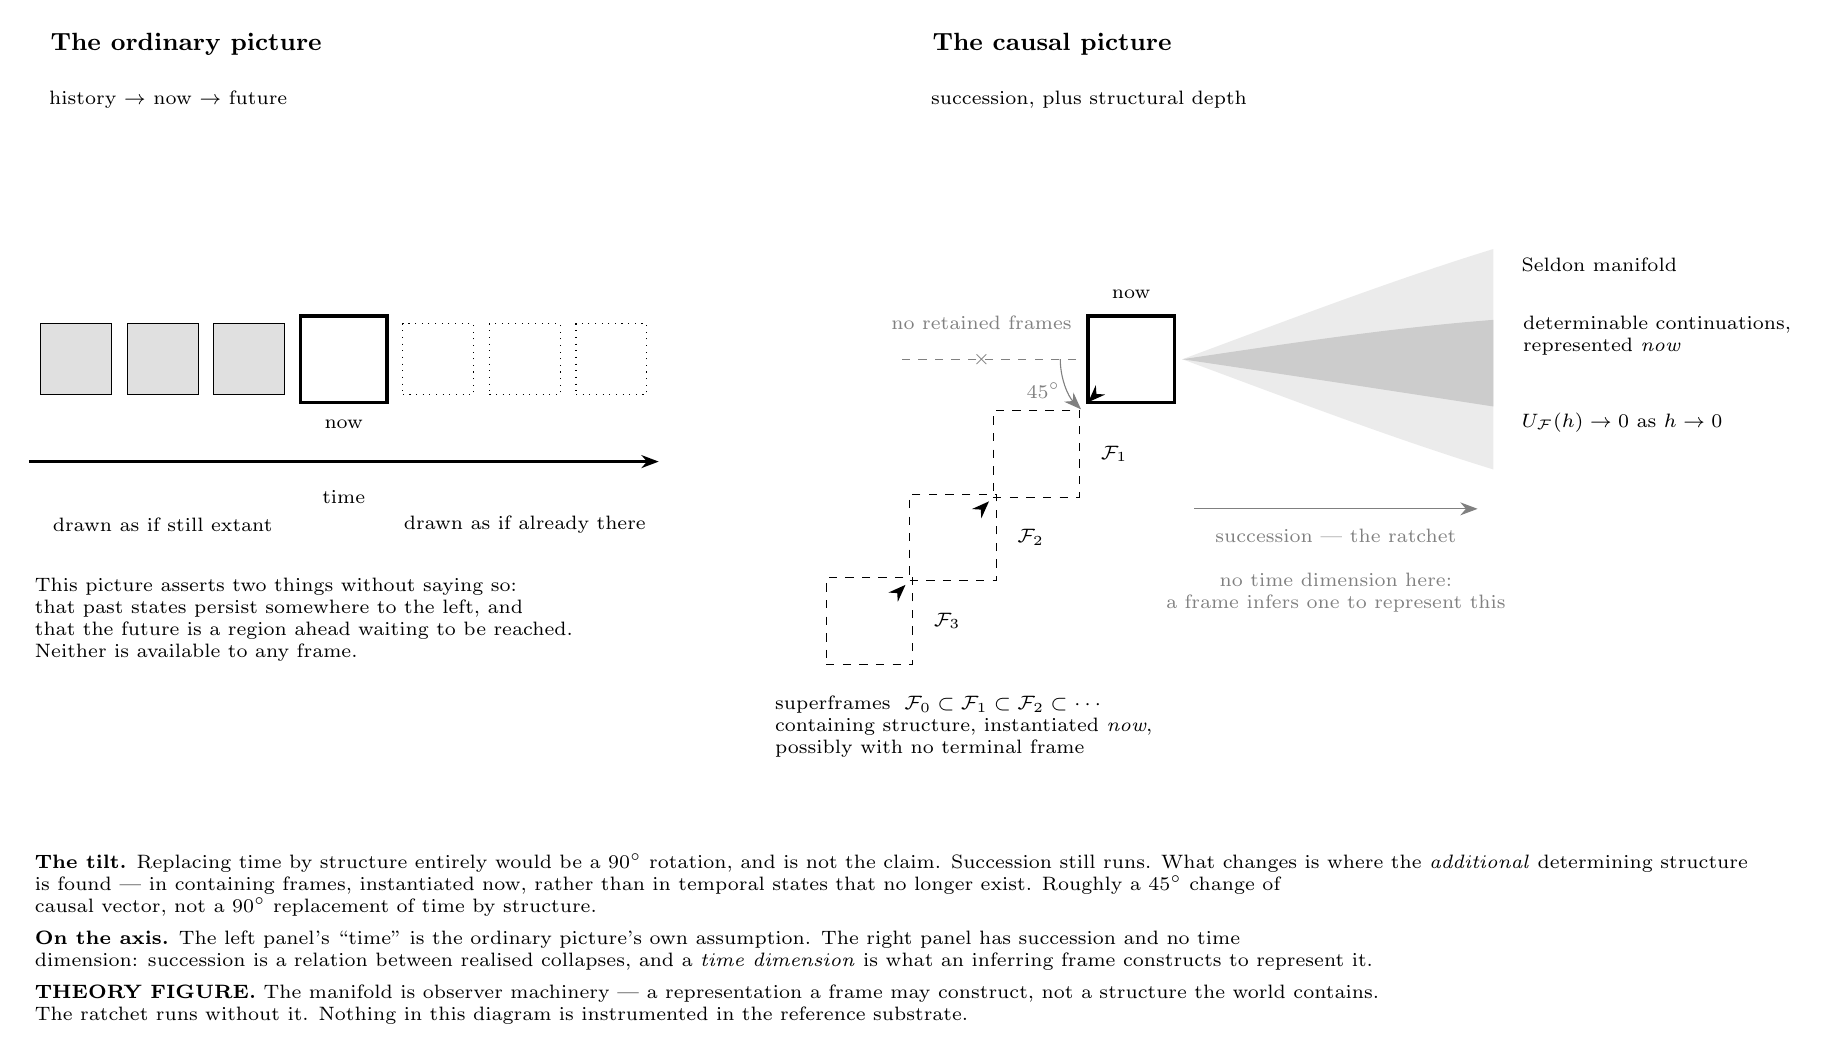
\begin{tikzpicture}[
  >={Stealth[length=2.2mm]},
  now/.style={draw, very thick, minimum size=11mm, inner sep=0pt},
  past/.style={draw, fill=black!12, minimum size=9mm, inner sep=0pt},
  fut/.style={draw, dotted, minimum size=9mm, inner sep=0pt},
  sup/.style={draw, dashed, minimum size=11mm, inner sep=0pt},
  lbl/.style={font=\scriptsize, inner sep=1.5pt},
  hd/.style={font=\small\bfseries, inner sep=2pt},
  note/.style={font=\scriptsize, align=left, inner sep=2pt},
  x=1mm, y=1mm,
]

%% ======================= LEFT: the ordinary picture ====================
\begin{scope}
  \node[hd, anchor=west] at (-34,40) {The ordinary picture};
  \node[lbl, anchor=west] at (-34,33) {history $\rightarrow$ now $\rightarrow$ future};

  \foreach \x in {-30,-19,-8}{\node[past] at (\x,0) {};}
  \node[now] (n) at (4,0) {};
  \node[lbl, below=1.4mm of n] {now};
  \foreach \x in {16,27,38}{\node[fut] at (\x,0) {};}

  \draw[->, thick] (-36,-13) -- (44,-13);
  \node[lbl] at (4,-17.5) {time};

  \node[lbl] at (-19,-21) {drawn as if still extant};
  \node[lbl] at (27,-21) {drawn as if already there};

  \node[note, anchor=north west] at (-36,-27)
    {This picture asserts two things without saying so:\\
     that past states persist somewhere to the left, and\\
     that the future is a region ahead waiting to be reached.\\
     Neither is available to any frame.};
\end{scope}

%% ======================= RIGHT: the causal picture =====================
\begin{scope}[shift={(104,0)}]
  \node[hd, anchor=west] at (-26,40) {The causal picture};
  \node[lbl, anchor=west] at (-26,33) {succession, plus structural depth};

  \node[now] (n2) at (0,0) {};
  \node[lbl, above=1.4mm of n2] {now};

  % --- the manifold ahead ---------------------------------------------
  \fill[black!8] (6.5,0) .. controls (20,5) and (33,10) .. (46,14)
    -- (46,-14) .. controls (33,-10) and (20,-5) .. (6.5,0) -- cycle;
  \fill[black!20] (6.5,0) .. controls (20,2) and (33,4) .. (46,5)
    -- (46,-6) .. controls (33,-4) and (20,-2) .. (6.5,0) -- cycle;
  \draw[->, gray] (8,-19) -- (44,-19);
  \node[lbl, gray, anchor=north] at (26,-21) {succession --- the ratchet};
  \node[lbl, gray, anchor=north, align=center] at (26,-26.5)
    {no time dimension here:\\a frame infers one to represent this};

  \node[lbl, anchor=west] at (49,12) {Seldon manifold};
  \node[note, anchor=west] at (49,3)
    {determinable continuations,\\represented \emph{now}};
  \node[lbl, anchor=west] at (49,-8) {$U_{\mathcal F}(h)\to0$ as $h\to0$};

  % --- where the past would be: nothing --------------------------------
  \draw[gray, dashed] (-7,0) -- (-30,0);
  \node[gray] at (-19,0) {\scriptsize$\times$};
  \node[note, anchor=south, gray] at (-19,3)
    {no retained frames};

  % --- superframes, down-left at 45 degrees ----------------------------
  \foreach \i/\d in {1/17, 2/32, 3/47}{
    \node[sup] (s\i) at (-\d*0.7071,-\d*0.7071) {};
    \node[lbl, anchor=west] at ($(s\i.east)+(2,0)$) {$\mathcal F_\i$};
  }
  \draw[->, thick, shorten >=1.4mm, shorten <=1.4mm] (n2) -- (s1);
  \draw[->, thick, shorten >=1.4mm, shorten <=1.4mm] (s1) -- (s2);
  \draw[->, thick, shorten >=1.4mm, shorten <=1.4mm] (s2) -- (s3);

  % --- the tilt, marked between the two rays ---------------------------
  \draw[gray, ->] (-9,0) arc (180:225:9);
  \node[lbl, gray, anchor=north east] at (-8.4,-2.4) {$45^{\circ}$};

  \node[note, anchor=north west] at (-46,-42)
    {superframes $\;\mathcal F_0\subset\mathcal F_1\subset\mathcal F_2\subset\cdots$\\
     containing structure, instantiated \emph{now},\\
     possibly with no terminal frame};
\end{scope}

%% ======================= shared caption ================================
\node[note, anchor=north west] at (-36,-62)
  {\textbf{The tilt.} Replacing time by structure entirely would be a
   $90^{\circ}$ rotation, and is not the claim. Succession still runs. What
   changes is where the \emph{additional} determining structure\\
   is found --- in containing frames, instantiated now, rather than in temporal
   states that no longer exist. Roughly a $45^{\circ}$ change of\\
   causal vector, not a $90^{\circ}$ replacement of time by structure.\\[1.2mm]
   \textbf{On the axis.} The left panel's ``time'' is the ordinary picture's own
   assumption. The right panel has succession and no time\\
   dimension: succession is a relation between realised collapses, and a
   \emph{time dimension} is what an inferring frame constructs to represent it.\\[1.2mm]
   \textbf{THEORY FIGURE.} The manifold is observer machinery --- a
   representation a frame may construct, not a structure the world contains.\\
   The ratchet runs without it. Nothing in this diagram is instrumented in the
   reference substrate.};
\end{tikzpicture}
}
\caption{The ordinary picture of time against the causal picture. Left: past
states drawn as though still extant and the future drawn as a region already
there --- neither of which any frame holds. Right: succession forward,
structural depth through containing frames at roughly $45^{\circ}$, and the
manifold as observer machinery ahead of the present.}
\label{fig:tilt}
\end{figure}

This matters for what an explanation is permitted to assume. A theory that located determining structure in earlier temporal states would require arbitrarily deep access to a past that no frame holds. Locating it in containing frames requires only structure that is instantiated now.

\section{Positioning and novelty}\label{sec:positioning}

The paper's relationship to established work can be summarised as follows.

\begin{description}[leftmargin=*,style=nextline]
\item[Established prior art.] Reachable sets, viability kernels, invariant and capture sets, dynamic programming, model-predictive feasible sets, Hamilton--Jacobi reachability, adaptive numerical resolution, and option value under irreversibility are established \citep{bellman1957,aubin1991,mitchell2005,berger1984,arrow1974,rawlings2017}.
\item[Structural synthesis.] The Seldon manifold treats these set-valued future structures as a frame-relative representation generated downstream of deterministic Graphic Equalisation and evaluated only on instantiated dimensions at operative discrete resolution.
\item[Specific contributions.] The terminology and formal roles of the Seldon manifold and Muchness; the explicit separation of local admissibility, counterfactual reachable geometry, deterministic collapse, Muchness, and Narrativium; dimension-instantiation discipline (NULL is not zero); and the decision-relevant reachability-compression hypothesis are claims of this framework.
\end{description}

It is worth being precise about the difference from a reachable set specifically, since that is the
nearest established object and the one a reader will substitute if the distinction is not drawn.

A reachable set is an extent, and membership in it is binary: a state is attainable within the
horizon or it is not. On the account given here that extent is the \emph{support} of the structure
rather than the structure --- the manifold is that support together with the fields of
Sections~\ref{sec:contours} over it, and the fields carry what the extent cannot. Three differences
follow, in increasing order of how badly the substitution misleads.

The fields are graded where membership is binary, and the grading is not a refinement of the
membership question but a replacement for it. Surviving structure prices continuations rather than
removing them, so a continuation whose price exceeds anything a frame can pay remains in the set and
is excluded by cost, not by admissibility. A reachable set has no way to represent that state of
affairs, and a construction that only computed extents would be answering a question this account
holds to be the wrong one.

The manifold carries where a frame \emph{goes}, not only where it \emph{could}. An extent is
indifferent between its members; a cost field has a descent direction, so the construction projects
an uninterrupted trajectory rather than merely bounding one. That is a different kind of prediction
and is what makes basins, lock-in and the horizon expressible at all.

And the manifold prices its own modification. A reachable set is computed for a system taken as
given; deformability is a field over the same manifold recording what altering the generating
structure would cost, so the representation includes the terms on which it can itself be changed.
This is the point at which the object stops resembling a reachability computation, because the
recursion --- landscape, cost of re-shaping it, cost of changing that --- is internal to the
construction rather than external to it, and is bounded by the same finite capacity throughout.

A fourth difference is about use rather than structure. A reachable set answers a question of
\emph{possibility} and carries no preference at all; what is done with it is left entirely outside.
A manifold carrying fields supports a decision, and supports more than one: a frame may hold a
non-dominated position across its fields, or satisfice on an acceptable region and act only on
projected departure, or scalarise into a single objective where it has one. Which discipline applies
is the frame's, not the construction's, and the paper claims none of them as its own --- each is
established work, and the acceptable-region form in particular is developed in the viability
literature this paper already depends on. What the construction contributes is the object the
discipline runs on: the fields, frame-represented and unscalarised unless the frame scalarises them.

It is worth being explicit about how much of this belongs to that literature, since the answer is
more than it is comfortable to concede. Holding a control constant while the region is respected,
acting only where it would cease to be, and acting then by the pointwise-minimal admissible change is
Aubin's \emph{inertia principle}, and the resulting trajectories his \emph{heavy viable solutions}
\citep{aubinfrankowska1989,aubin1991,aubinbayen2011}; the engineering form, acting on a projected
rather than observed departure, is self-triggered control \citep{tabuada2007,heemels2012}. That the trigger
is \emph{projected} rather than measured is what makes the forward structure necessary rather than
ornamental: a discipline that waits for observed departure needs a boundary test on the current
state and nothing more, and would not require a manifold at all. Acting on a projection is what buys
the interval in which cheap options still exist, and it is also what exposes the discipline to being
wrong in a way a measured trigger is not --- the projection may be mistaken, and acting on it spends
capacity that a frame with a better manifold would have kept. Nor do
the obvious extensions escape it. A constraint region that changes over time, or co-evolves with the
system it constrains, is treated there as a viability tube and by mutational analysis
\citep{aubin1999}; and responding by altering the dynamics rather than steering within them is
native to it as well, through viability multipliers and the promotion of fixed coefficients into
controls \citep{aubinbayen2011}. The re-shaping of a landscape, which might have looked like this
construction's own contribution, is not.

What is left is narrower and is epistemic rather than mathematical. In that literature the
constraint region is a given of the model --- it may vary, it may co-evolve --- but it is not a
representation the frame holds and may have wrong. There is no residual between the region as
represented and the region as it is, and so no mechanism by which a frame discovers its own
constraints were mis-specified and revises them, which is what the substrate's residual and minting
machinery supplies. That is a claim about where the region comes from rather than about what to do
once it is given, and it should be weighed knowing that adaptive and learning-based treatments of
safe control press on exactly this point.

Stated positively rather than by subtraction, what the construction offers is machinery for seeing
the shape of a frame's potential futures and then working on that shape: not a method for reaching
an outcome, but a representation general enough to carry whichever outcomes a frame holds and
whichever discipline it applies to them. Its generality is its content. It fixes no fields, since
those are what the frame instantiates; it fixes no objective, since acceptability is represented
rather than given; and it fixes no rule for acting, since holding a region, ranking by dominance and
scalarising are all available to a frame that represents what it needs to. And because the
acceptable region is itself represented, what a frame is optimising for is as revisable as how it
gets there --- which is the same point as the epistemic one above, seen from the other side.

None of which displaces the established work: where the question genuinely is one of extent, the
existing machinery answers it and answers it better, and the fields above are defined over exactly
the sets that machinery computes. The claim is not that these tools are insufficient for their own
question, nor that the decision disciplines above are this paper's --- they are not. It is narrower:
that a frame acting on its own future needs fields over the reachable set and not only the set, that
which fields those are is its own affair, and that among them may be one pricing the alteration of
the rest.

\section{Falsifiability commitments}\label{sec:falsifiability}

\begin{enumerate}[leftmargin=*]
\item \textbf{Cost contours and basins.} Fails if the continuations a frame actually takes, absent intervention, are not the cheap ones --- if the descent direction of the cost field does not predict where an uninterrupted frame goes --- or if persistence in a region can be exhibited with no corresponding basin, or a basin with no corresponding persistence. It fails also if deformation cost is uniform across every manifold in every grounding, so that no location ever offers a cheaper change with a larger effect than another. And it fails if the two fields cannot come apart --- if expected capacity after an action is always the capacity before it less the cost, so that no expensive continuation ever raises capacity and no cheap one lowers it. (The claim is about the fields' shape relative to a frame's capacity, not about the values of any metric over them.)
\item \textbf{Deterministic counterfactual typing.} Fails if the Seldon construction requires multiple fundamentally random realised outcomes from one causally complete antecedent rather than multiple deterministic continuations under differing represented future conditions.
\item \textbf{Reachability utility.} Fails for a claimed task class if reachable geometry cannot preserve distinctions needed for prediction or control that trajectory-level representation preserves.
\item \textbf{Dimension/value typing.} Fails if an absent future dimension must be represented as the numerical value zero rather than remaining undefined until instantiated.
\item \textbf{Adaptive resolution.} Fails as an efficiency hypothesis if decision-directed refinement gives no advantage over uniform refinement in the claimed class.
\item \textbf{Muchness distinction.} Fails if retained distinguishable possibility and capacity to deform that possibility cannot be independently varied in any grounding.
\item \textbf{Irreversibility.} Fails for a claimed grounding if supposedly deleted reachable distinctions are always restorable without crossing an additional constraint or expending additional compatible capability.
\item \textbf{Reachability compression.} Fails if explicit trajectory representations consistently achieve equal or lower decision-relevant description cost for the claimed task families.
\end{enumerate}

\section{Conclusion}\label{sec:conclusion}

Graphic Equalisation supplies deterministic admissible continuation and collapse. The Seldon manifold is the structured geometry of unrealised counterfactual continuation that remains reachable:
\[
\boxed{
\Gamma
\rightarrow
\text{admissible possibility}
\rightarrow
\Seldon
\rightarrow
\text{reachable geometry}
\xrightarrow{\mathcal C}
\text{realised history}.
}
\]

The distinction between reachable geometry and realised history is essential: the manifold contains counterfactual futures because the frame has not fixed all future interventions and containing conditions, not because the Graph Law is stochastic.

The future, in this framework, is not primarily a destination. It is a reachable geometry.

\begin{thebibliography}{99}

\bibitem[Arrow and Fisher(1974)]{arrow1974}
Kenneth J. Arrow and Anthony C. Fisher.
\newblock Environmental preservation, uncertainty, and irreversibility.
\newblock \emph{The Quarterly Journal of Economics}, 88(2):312--319, 1974.
\newblock doi:10.2307/1883074.

\bibitem[Aubin and Frankowska(1989)]{aubinfrankowska1989}
Jean-Pierre Aubin and H\'el\`ene Frankowska.
\newblock \emph{Dynamic Regulation of Controlled Systems, Inertia Principle and Heavy Viable Solutions}.
\newblock IIASA Working Paper WP-89-086, Laxenburg, 1989.

\bibitem[Aubin(1990)]{aubin1990}
Jean-Pierre Aubin.
\newblock A survey of viability theory.
\newblock \emph{SIAM Journal on Control and Optimization}, 28(4):749--788, 1990.
\newblock doi:10.1137/0328044.

\bibitem[Aubin(1999)]{aubin1999}
Jean-Pierre Aubin.
\newblock \emph{Mutational and Morphological Analysis: Tools for Shape Evolution and Morphogenesis}.
\newblock Birkh\"auser, Boston, 1999.

\bibitem[Aubin(1991)]{aubin1991}
Jean-Pierre Aubin.
\newblock \emph{Viability Theory}.
\newblock Birkh\"auser, Boston, 1991.

\bibitem[Aubin et al.(2011)]{aubinbayen2011}
Jean-Pierre Aubin, Alexandre M. Bayen, and Patrick Saint-Pierre.
\newblock \emph{Viability Theory: New Directions}.
\newblock Springer, Berlin, 2nd edition, 2011.

\bibitem[Heemels et al.(2012)]{heemels2012}
W. P. M. H. Heemels, K. H. Johansson, and P. Tabuada.
\newblock An introduction to event-triggered and self-triggered control.
\newblock In \emph{Proceedings of the 51st IEEE Conference on Decision and Control}, pages 3270--3285, 2012.

\bibitem[Tabuada(2007)]{tabuada2007}
Paulo Tabuada.
\newblock Event-triggered real-time scheduling of stabilizing control tasks.
\newblock \emph{IEEE Transactions on Automatic Control}, 52(9):1680--1685, 2007.

\bibitem[Bansal et~al.(2017)Bansal, Chen, Herbert, and Tomlin]{bansal2017}
Somil Bansal, Mo Chen, Sylvia Herbert, and Claire J. Tomlin.
\newblock Hamilton--Jacobi reachability: A brief overview and recent advances.
\newblock In \emph{2017 IEEE 56th Annual Conference on Decision and Control}, pages 2242--2253, 2017.

\bibitem[Bellman(1957)]{bellman1957}
Richard Bellman.
\newblock \emph{Dynamic Programming}.
\newblock Princeton University Press, Princeton, 1957.

\bibitem[Berger and Oliger(1984)]{berger1984}
Marsha J. Berger and Joseph Oliger.
\newblock Adaptive mesh refinement for hyperbolic partial differential equations.
\newblock \emph{Journal of Computational Physics}, 53(3):484--512, 1984.
\newblock doi:10.1016/0021-9991(84)90073-1.

\bibitem[Cunis and Kolmanovsky(2021)]{cunis2021}
Torbj\o rn Cunis and Ilya Kolmanovsky.
\newblock Viability, viscosity, and storage functions in model-predictive control with terminal constraints.
\newblock \emph{Automatica}, 131:109748, 2021.

\bibitem[Dixit and Pindyck(1994)]{dixit1994}
Avinash K. Dixit and Robert S. Pindyck.
\newblock \emph{Investment under Uncertainty}.
\newblock Princeton University Press, Princeton, 1994.

\bibitem[Henry(1974)]{henry1974}
Claude Henry.
\newblock Investment decisions under uncertainty: The ``irreversibility effect.''
\newblock \emph{American Economic Review}, 64(6):1006--1012, 1974.

\bibitem[Maidens et~al.(2013)Maidens, Kaynama, Mitchell, Oishi, and Dumont]{maidens2013}
John N. Maidens, Shahab Kaynama, Ian M. Mitchell, Meeko M. K. Oishi, and Guy A. Dumont.
\newblock Lagrangian methods for approximating the viability kernel in high-dimensional systems.
\newblock \emph{Automatica}, 49(7):2017--2029, 2013.
\newblock doi:10.1016/j.automatica.2013.03.020.

\bibitem[Mitchell et~al.(2005)Mitchell, Bayen, and Tomlin]{mitchell2005}
Ian M. Mitchell, Alexandre M. Bayen, and Claire J. Tomlin.
\newblock A time-dependent Hamilton--Jacobi formulation of reachable sets for continuous dynamic games.
\newblock \emph{IEEE Transactions on Automatic Control}, 50(7):947--957, 2005.
\newblock doi:10.1109/TAC.2005.851439.

\bibitem[Rawlings et~al.(2017)Rawlings, Mayne, and Diehl]{rawlings2017}
James B. Rawlings, David Q. Mayne, and Moritz M. Diehl.
\newblock \emph{Model Predictive Control: Theory, Computation, and Design}.
\newblock Nob Hill Publishing, 2nd edition, 2017.

\bibitem[Rissanen(1978)]{rissanen1978}
Jorma Rissanen.
\newblock Modeling by shortest data description.
\newblock \emph{Automatica}, 14(5):465--471, 1978.
\newblock doi:10.1016/0005-1098(78)90005-5.

\bibitem[Szolnoki(2000)]{szolnoki2000}
Dietmar Szolnoki.
\newblock Viability kernels and control sets.
\newblock \emph{ESAIM: Control, Optimisation and Calculus of Variations}, 5:175--185, 2000.

\end{thebibliography}

\end{document}
